%% \begin{document}

%% 引数 : 年度,タイトル,学籍番号,氏名

%% 卒論中間発表
\mktitlebmid{2}{顕著性マップに基づいたドライバの視線予測モデル}
             {17-1-837-0014}{本間 友也}

%% 卒論
%%\mktitleb{}{}
%%          {}{}

%% %% 修論中間発表
%% \mktitlemmid{}{}
%%             {}{}

%% %% 修論
%% \mktitlem{}{}
%%          {}{}

\section{概要}
\vspace{-1mm}
昨今の自動車業界では,自動運転技術と並行してドライバのサポート技術の開発も進められている.
その一つにヘッドアップディスプレイによる新たな情報表示技術がある.
しかし,この技術には運転の妨げとなる危険性も指摘されていることから,安全に配慮した情報表示デザインを検討するために,
ドライバの視線を予測するシミュレーション技術の開発が望まれている.
ドライバの視線を予測する技術として,小玉らの顕著性マップを応用した数理モデル\cite{Kodama}が挙げられる.
小玉らのモデルは,Ittiらの顕著性マップ\cite{Itti}に対して,
初期視覚系受容野における中心周辺拮抗型の空間差分や視覚的順応をもたらす時間応答特性,
および高次の運動検出機構による特徴抽出を考慮して拡張を施したものである.
しかしながら,交差点進入時のような低速走行時において視線の推定精度が低下するという課題が残されている.
この原因としては,運動検出機構における速度算出過程での時間差分間隔が固定されていることにあると考えられる.
そこで本研究では,小玉らのモデルにおける低速走行時の視線推定精度を向上させることを目的とし,
運動ベクトルの算出過程に走行速度が反映されるような修正と,モデルの再構築を行う.
本報告では,顕著性マップ理論を理解するためにIttiらの顕著性マップモデルの構築に取り組んだ結果,従来モデルを再構築した結果,および運動ベクトルの演算方法について述べる.

\vspace{-3mm}

\section{顕著性マップモデル}
\vspace{-2mm}
\subsection{Ittiらのモデル}

Ittiらのモデルは,視覚系の初期に処理される色,傾き,輝度といった基本的な画像特徴量に基づき,
注意の向けられやすさに相当する顕著さを算出するモデルである.

\subsection{小玉らのモデル}
小玉らのモデルは,初期視覚系受容野特性や視覚的順応特性などを導入してIttiらの顕著性マップモデルに拡張を施した数理モデルであり,
動画のフレーム間差分を算出することで,運動特徴量を検出する機構を持たせている.
小玉らのモデルを図\ref{fig:kodama}に示す.小玉らのモデルでは先述した課題の他にも,出力画像に対してフレームごとに正規化処理を行うため,
異なるシーン間での顕著さを比較できないなどといった問題も抱えている.

%\newpage
\begin{figure}[h]
 \centering
 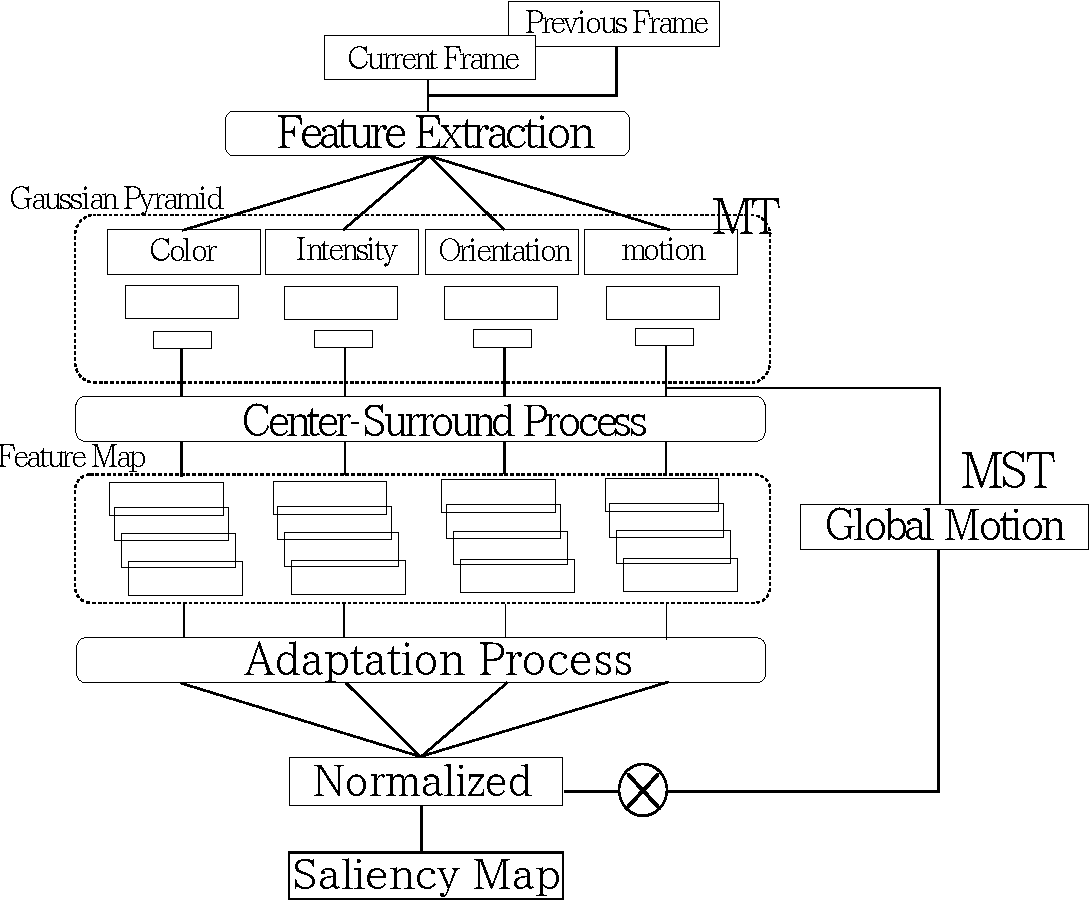
\includegraphics[keepaspectratio,width=92mm]{./fig/saliency_kodama_model.pdf}
 \centering
  \caption{小玉らのモデル}
 \label{fig:kodama}
\end{figure}
\vspace*{-6mm}

\section{シミュレーション結果}
\vspace{-3.2mm}
\subsection{顕著性マップモデルのシミュレーション結果}
まず,小玉らのモデルの基礎となるIttiらのモデルを再現した.シミュレーション結果を図\ref{fig:itti_saliency}に示す.
\vspace{-1.2mm}
\begin{figure}[h]
    \begin{minipage}[h]{0.5\hsize}
      \centering
      \includegraphics[width=0.98\textwidth]{./fig/001.eps}
      \subcaption{入力画像}
      \label{fig:input}
    \end{minipage}
    \begin{minipage}[h]{0.5\hsize}
      \centering
      \includegraphics[width=0.98\textwidth]{./fig/saliency_color_normalize.eps}
      \subcaption{算出した顕著性マップ}
      \label{fig:output}
    \end{minipage}
    \vspace{0.5mm}
    \caption{Ittiらのモデルの再現結果}
    \label{fig:itti_saliency}
\end{figure}

\vspace{-2mm}

次に,従来の小玉らのモデルを一部改良し,正規化アルゴリズムの変更を行った.
シミュレーション結果を図\ref{fig:kodama_saliency}に示す.
正規化アルゴリズムを変更することで,異なるフレーム間での顕著さの比較が可能となった.
\vspace{-1.0mm}
\begin{figure}[h]
    \begin{minipage}[h]{0.5\hsize}
      \centering
      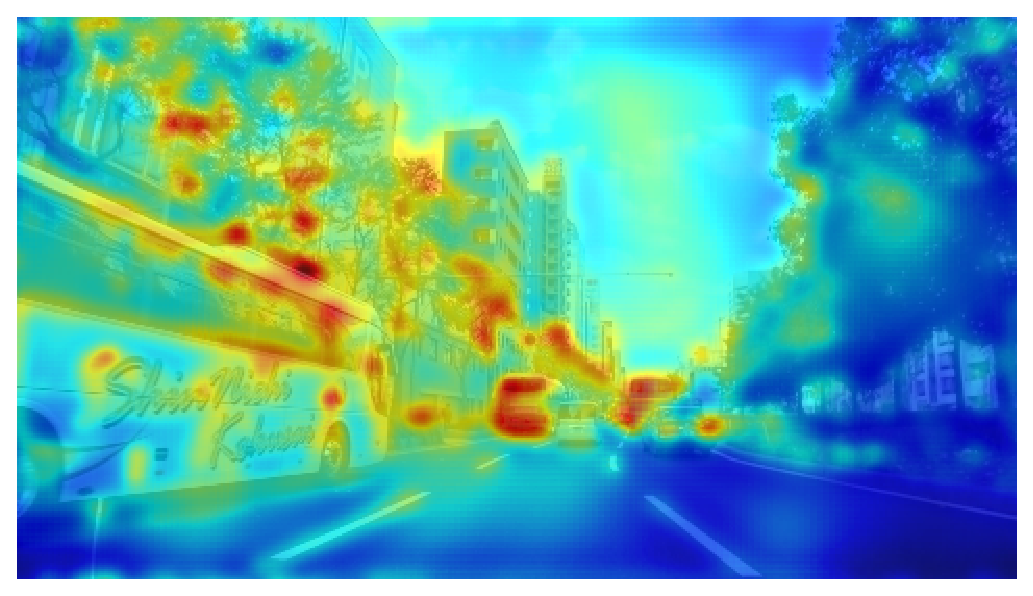
\includegraphics[width=0.98\textwidth]{./fig/132_before.eps}
      \label{fig:kodama_before}
    \end{minipage}
    \begin{minipage}[h]{0.5\hsize}
      \centering
      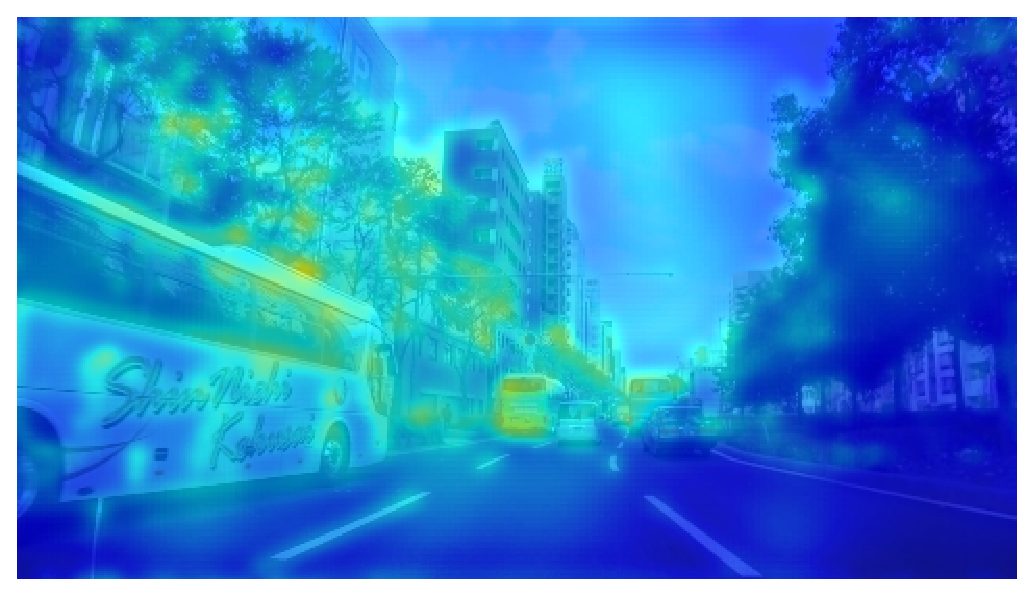
\includegraphics[width=0.98\textwidth]{./fig/132_after.eps}
      \label{fig:kodama_after}
    \end{minipage}
    \begin{minipage}[h]{0.5\hsize}
      \centering
      \vspace{-3.2mm}
      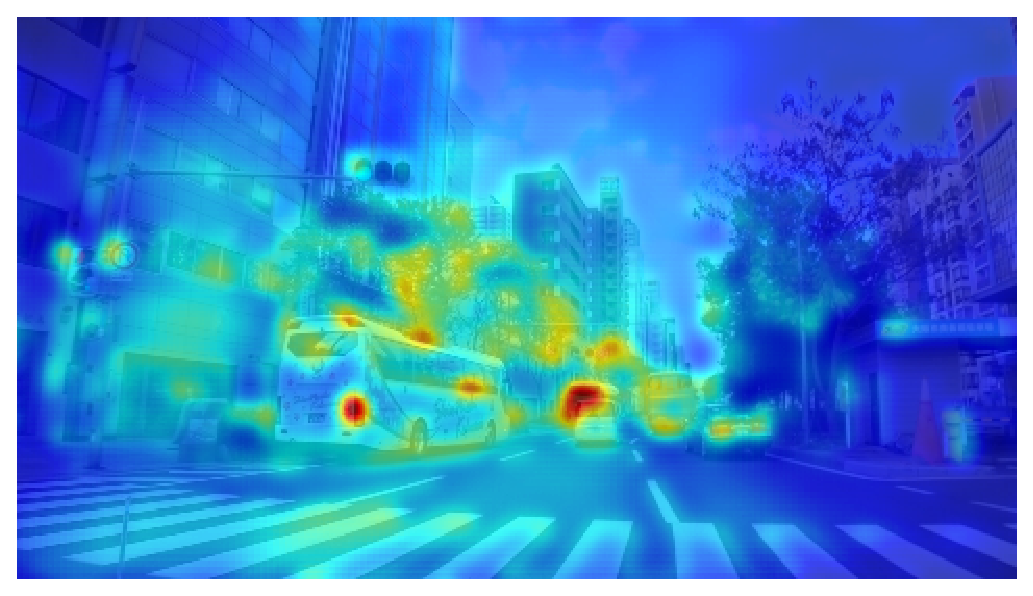
\includegraphics[width=0.98\textwidth]{./fig/101_before.eps}
      \subcaption{小玉らのモデルの出力}
      \label{fig:kodama_before}
    \end{minipage}
    \begin{minipage}[h]{0.5\hsize}
      \centering
      \vspace{-3.2mm}
      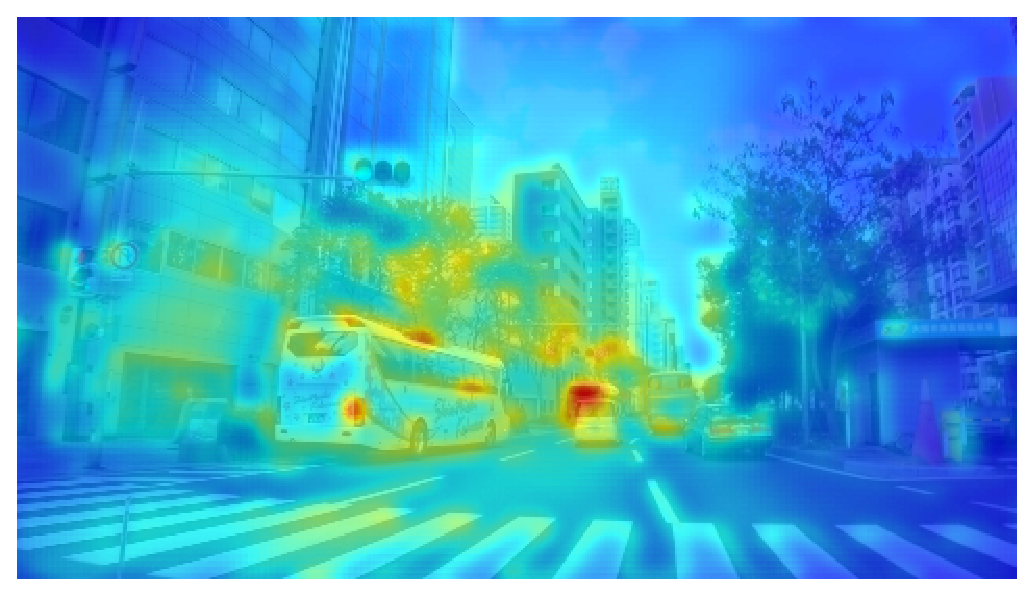
\includegraphics[width=0.98\textwidth]{./fig/101_after.eps}
      \subcaption{改良版モデルの出力}
      \label{fig:kodama_after}
    \end{minipage}
    \vspace*{0.8mm}
    \caption{小玉らのモデルの再現と改良結果}
    \label{fig:kodama_saliency}
\end{figure}

%\vspace{-0.5mm}
\subsection{運動ベクトルの演算結果}
小玉らのモデルを再構築するに際して,特徴点の運動ベクトルの演算について検討した.
代表的な特徴点検出法であるSIFT\cite{sift}を用いて特徴点を検出して特徴点マッチングを施し,その運動ベクトルを求めた結果を図\ref{fig:sift}に示す.

\vspace{-1.5mm}

\begin{figure}[h]
  \centering
  \includegraphics[keepaspectratio,width=80mm]{./fig/matching_movie_sift.eps}
  \centering
  \vspace{0.5mm}
  \caption{SIFTを用いた特徴点マッチングの結果}
  \label{fig:sift}
\end{figure}

\vspace{-3.5mm}

\section{まとめと今後の展望}
\vspace{-2.0mm}
本稿では,小玉らのモデルのベースとなる,顕著性マップモデルの構築と小玉らのモデルの正規化アルゴリズムの変更,および運動ベクトル演算を行った.
今後は,小玉らのモデルの運動検出アルゴリズムをSIFTなどの特徴量検出アルゴリズムを用いたものに変更し,モデルの予測精度の向上を図る.
また,モデルの再構築も引き続き行う.

\vspace{-4.0mm}
%%%%%%%%%%%%% 参考文献 %%%%%%%%%%%%
\begin{thebibliography}{}
\vspace{-1.5mm}
\scriptsize{
\bibitem{Kodama}
M.Kodama et al.:"A saliency based motion detection model of visual system consideringvisual adaptation properties",\\IEEE(EMBS),37,pp.6658-6661(2015)
\bibitem{Itti}
L.Itti et al.:"A model of saliency-based visual attention for rapid scene analysis",IEEE(PAMI),VOL.20,NO.11(1998)
\bibitem{sift}
D.G.Lowe:"Object~recognition~from~local~scale-invariant~features",\\IEEE(ICCV),pp.1150-1157(1999)
}
\end{thebibliography}
